\prob
{
    \begin{enumerate}[label=(\roman*)]
        \item   Find a maximum-weight spanning tree of the graph in the next figure. Is this the unique such tree?
                \begin{center}
                    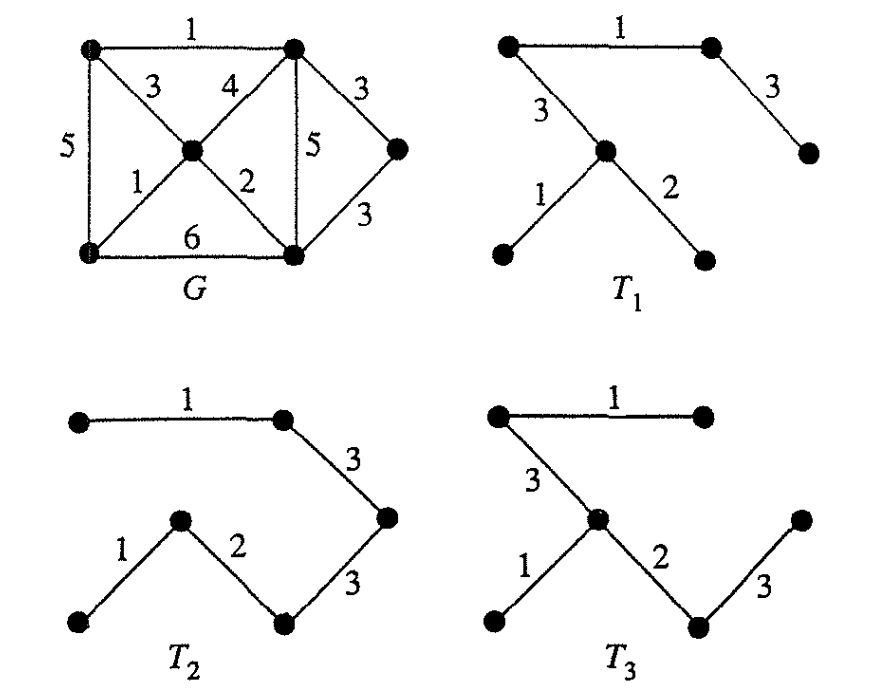
\includegraphics[width=8cm]{Test1/Problem14/Figure-i.png}
                \end{center}
                
        \item   Find all maximum-weight spanning trees and all minimum-weight spanning trees of the graph in the next
                figure, where the edge labels are interpreted as weights.
                \begin{center}
                    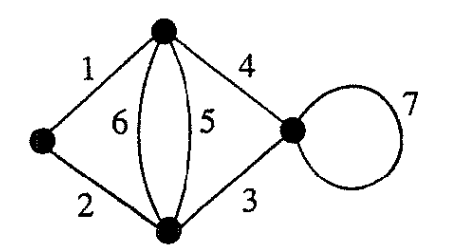
\includegraphics[width=4cm]{Test1/Problem14/Figure-ii.png}
                \end{center}
    \end{enumerate}
}
\begin{proof}
\begin{enumerate}
	\item 
            There are only 2 maximum-weight spanning trees of the graph. I have ilustrated what will greedy do step by step,
            and with all possible desicions being made.
            \begin{center}
                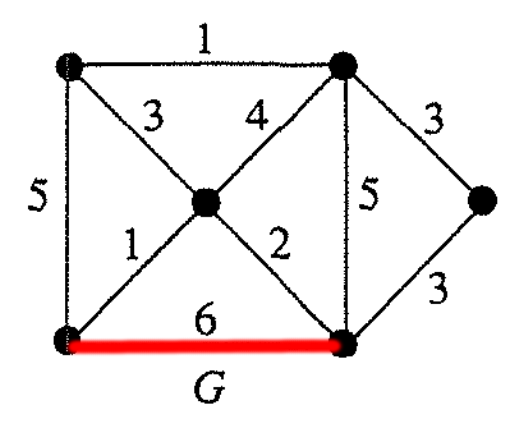
\includegraphics[width=4cm]{Test1/Problem14/Fig-i-1.png}
            \end{center}
            
            \begin{center}
                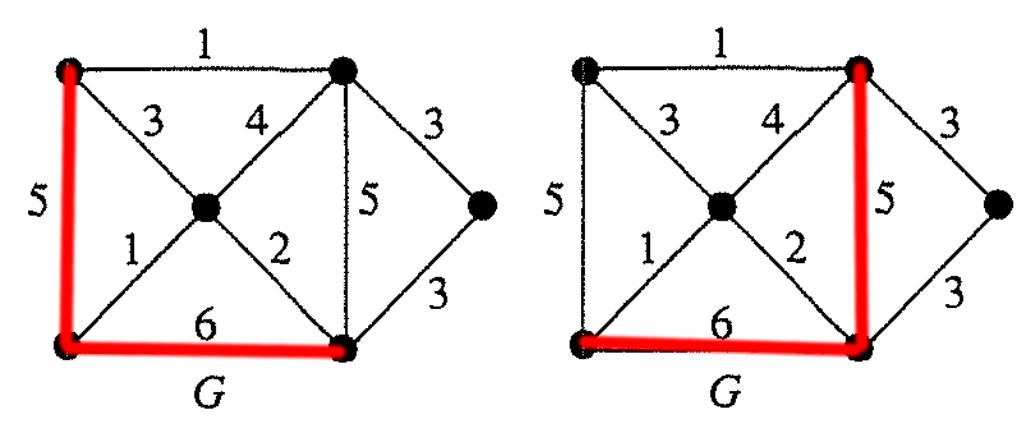
\includegraphics[width=8cm]{Test1/Problem14/Fig-i-2.png}
            \end{center}
            
            \begin{center}
                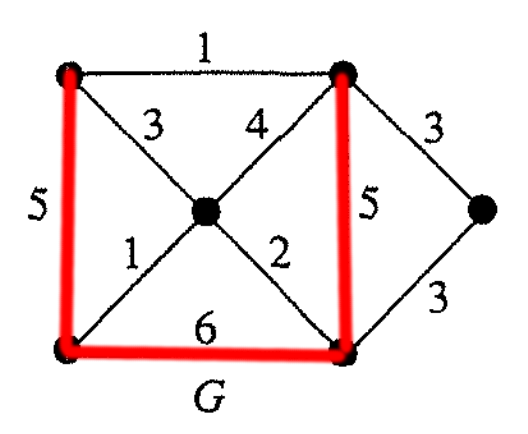
\includegraphics[width=4cm]{Test1/Problem14/Fig-i-3.png}
            \end{center}
            
            \begin{center}
                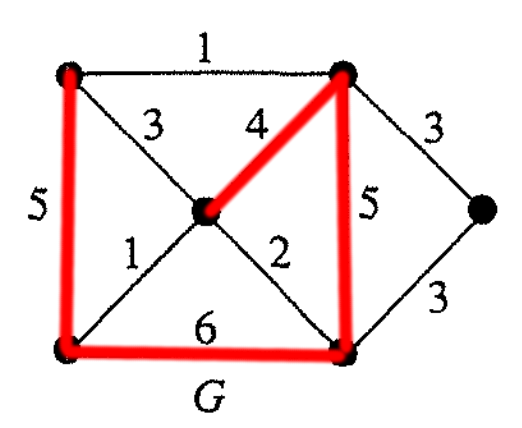
\includegraphics[width=4cm]{Test1/Problem14/Fig-i-4.png}
            \end{center}
            
            \begin{center}
                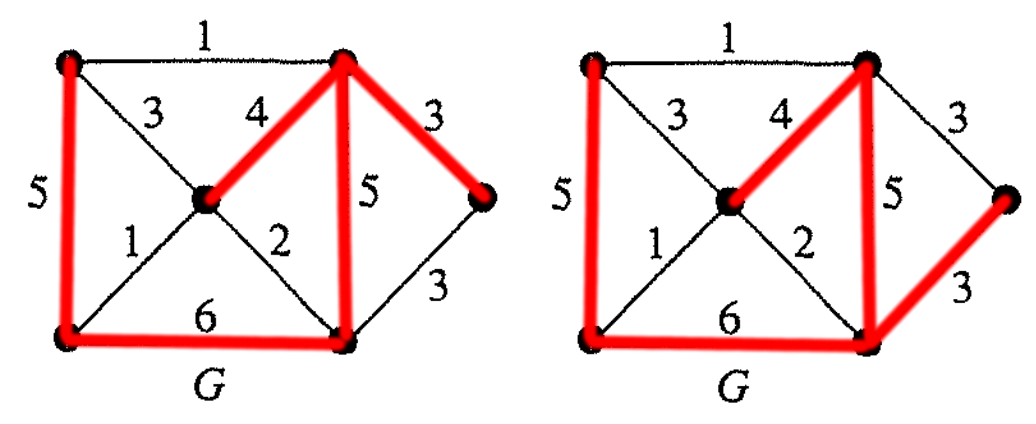
\includegraphics[width=8cm]{Test1/Problem14/Fig-i-5.png}
            \end{center}
    \item
            As the weight function is injective, the maximum-weight and minimum-weight spanning trees are unique.\pn
            
            Here is again an ilustration of what greedy would do in both scenarios.\pn
            
            Maximum-weight:\pn
            
            \begin{center}
                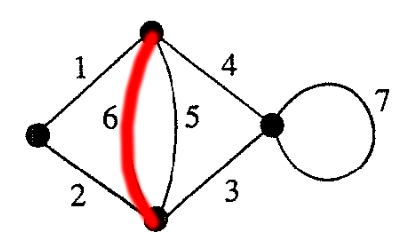
\includegraphics[width=5cm]{Test1/Problem14/Fig-ii-a-1.png}
            \end{center}
            
            \begin{center}
                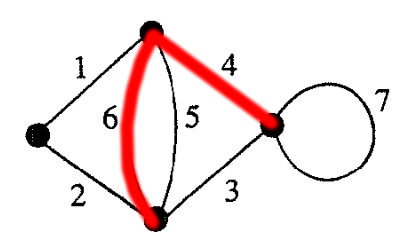
\includegraphics[width=5cm]{Test1/Problem14/Fig-ii-a-2.png}
            \end{center}
            
            \begin{center}
                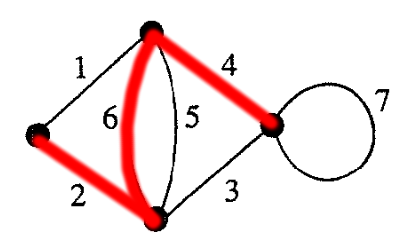
\includegraphics[width=5cm]{Test1/Problem14/Fig-ii-a-3.png}
            \end{center}     
                
            Minimum-weight:\pn
            
            \begin{center}
                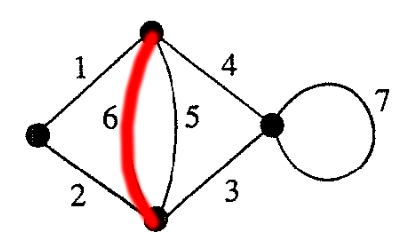
\includegraphics[width=5cm]{Test1/Problem14/Fig-ii-a-1.png}
            \end{center}
            
            \begin{center}
                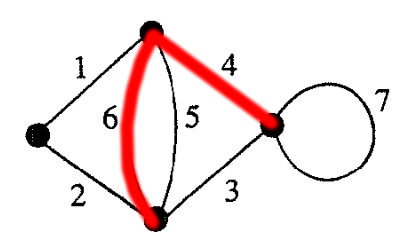
\includegraphics[width=5cm]{Test1/Problem14/Fig-ii-a-2.png}
            \end{center}
            
            \begin{center}
                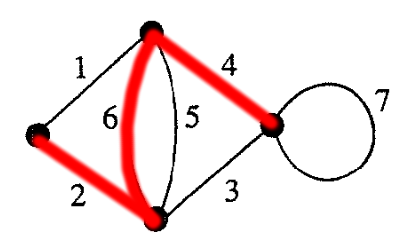
\includegraphics[width=5cm]{Test1/Problem14/Fig-ii-a-3.png}
            \end{center}
\end{enumerate}
\end{proof}